\section{Pemodelan Sistem Tiket}
\label{apx:analisis-kebutuhan}

Sebelum membahas pengoptimalan sistem tiket, perlu dibahas sistem tiket seperti apa yang ingin dioptimalkan pada penelitian ini. Oleh karena itu, berikut adalah spesifikasi sistem tiket yang dimaksud. Sistem ini merupakan pemodelan dari sistem tiket yang ada secara umum.

Berdasarkan studi yang sudah dibahas sebelumnya dan berdasarkan fokus yang ingin dibahas pada penelitian ini, komponen sistem yang relevan dengan penelitian ini adalah layanan pengguna, layanan tiket, dan layanan gerbang pembayaran.

\subsection{Layanan Pengguna}

Layanan ini merupakan layanan yang berkaitan dengan otentikasi pengguna, seperti registrasi dan login pengguna. Layanan ini menyimpan data pengguna sistem tiket yang merupakan pemesan.

\subsubsection{Kebutuhan Fungsional dan Non-Fungsional}

Kebutuhan fungsional layanan pengguna dibahas pada Tabel \ref{table:fungsional-pengguna}, sedangkan kebutuhan nonfungsional layanan pengguna dibahas pada Tabel \ref{table:nonfungsional-pengguna}.

\pagebreak

Berikut adalah kebutuhan fungsional layanan pengguna.

\begingroup
\footnotesize
\begin{longtable}{|l|p{0.4\textwidth}|p{0.4\textwidth}|}
    \caption{Kebutuhan Fungsional Layanan Pengguna}
    \label{table:fungsional-pengguna}                                                                                                                                                            \\
    \hline
    \textbf{ID} & \textbf{Kebutuhan}                                                                           & \textbf{Deskripsi}                                                              \\
    \endfirsthead

    \multicolumn{3}{|l|}{\tablename\ \thetable\ -- \textit{Lanjutan dari halaman sebelumnya}}                                                                                                    \\
    \hline
    \textbf{ID} & \textbf{Kebutuhan}                                                                           & \textbf{Deskripsi}                                                              \\
    \endhead

    \hline
    \multicolumn{3}{|r|}{\textit{Dilanjutkan ke halaman berikutnya}}                                                                                                                             \\
    \endfoot

    \hline
    \endlastfoot

    \hline
    UF-01       & Sistem dapat melayani registrasi pengguna.                                                   &                                                                                 \\
    \hline
    UF-02       & Sistem menyediakan mekanisme \textit{login} bagi pengguna.                                   &                                                                                 \\
    \hline
    UF-03       & Sistem menyediakan \textit{endpoint} untuk memperoleh informasi pengguna yang terotentikasi. & \textit{Endpoint} yang dapat digunakan oleh layanan lain seperti layanan tiket. \\
\end{longtable}
\endgroup

Berikut adalah kebutuhan non-fungsional layanan pengguna:

\begingroup
\footnotesize
\begin{longtable}{|l|p{0.4\textwidth}|p{0.4\textwidth}|}
    \caption{Kebutuhan Non-Fungsional Layanan Pengguna}
    \label{table:nonfungsional-pengguna}                                                                                                                                                                       \\
    \hline
    \textbf{ID} & \textbf{Parameter}   & \textbf{Kebutuhan}                                                                                                                                                    \\
    \endfirsthead

    \multicolumn{3}{|l|}{\tablename\ \thetable\ -- \textit{Lanjutan dari halaman sebelumnya}}                                                                                                                  \\
    \hline
    \textbf{ID} & \textbf{Parameter}   & \textbf{Kebutuhan}                                                                                                                                                    \\
    \endhead

    \hline
    \multicolumn{3}{|r|}{\textit{Dilanjutkan ke halaman berikutnya}}                                                                                                                                           \\
    \endfoot

    \hline
    \endlastfoot

    \hline
    UN-01       & Otentisitas Pengguna & Layanan lain dapat memverifikasi otentikasi token pengguna tanpa harus memanggil layanan pengguna, seperti dengan penggunaan token JWT dengan kunci rahasia tertentu. \\
\end{longtable}
\endgroup

\subsubsection{Entitas Layanan}

Entitas yang berkaitan dengan layanan ini adalah entitas pengguna (User). Entitas tersebut memiliki properti sebagaimana ditunjukkan pada Tabel \ref{table:skema-entitas-invoice}.

\begingroup
\footnotesize
\begin{longtable}{|l|p{0.2\textwidth}|p{0.4\textwidth}|}
    \caption{Skema Entitas Invoice}
    \label{table:skema-entitas-invoice}                                                       \\
    \hline
    \textbf{Atribut} & \textbf{Tipe Data} & \textbf{Deskripsi}                                \\
    \endfirsthead

    \multicolumn{3}{|l|}{\tablename\ \thetable\ -- \textit{Lanjutan dari halaman sebelumnya}} \\
    \hline
    \textbf{Atribut} & \textbf{Tipe Data} & \textbf{Deskripsi}                                \\
    \endhead

    \hline
    \multicolumn{3}{|r|}{\textit{Dilanjutkan ke halaman berikutnya}}                          \\
    \endfoot

    \hline
    \endlastfoot

    \hline
    id               & \texttt{string}    & ID unik untuk setiap pengguna.                    \\
    \hline
    name             & \texttt{string}    & Nama pengguna.                                    \\
    \hline
    email            & \texttt{string}    & Alamat surel pengguna.                            \\
    \hline
    password         & \texttt{string}    & Hash kata sandi pengguna                          \\
\end{longtable}
\endgroup


\pagebreak

\subsection{Layanan Tiket}

Layanan tiket memproses setiap permintaan yang berkaitan dengan pemesanan tiket. Layanan ini dapat dipecah menjadi beberapa layanan bergantung pada desain setiap arsitektur solusi.

\subsubsection{Kebutuhan Fungsional dan Non-Fungsional}

Berikut adalah kebutuhan fungsional layanan tiket:

\begingroup
\footnotesize
\begin{longtable}{|l|p{0.4\textwidth}|p{0.4\textwidth}|}
    \caption{Kebutuhan Fungsional Layanan Tiket}                                                                                                                                                                                                                                                                                                                                                                                                                                                             \\
    \hline
    \textbf{ID} & \textbf{Kebutuhan}                                                                                                                                                                                   & \textbf{Deskripsi}                                                                                                                                                                                                                                                                  \\
    \endfirsthead

    \multicolumn{3}{|l|}{\tablename\ \thetable\ -- \textit{Lanjutan dari halaman sebelumnya}}                                                                                                                                                                                                                                                                                                                                                                                                                \\
    \hline
    \textbf{ID} & \textbf{Kebutuhan}                                                                                                                                                                                   & \textbf{Deskripsi}                                                                                                                                                                                                                                                                  \\
    \endhead

    \hline
    \multicolumn{3}{|r|}{\textit{Dilanjutkan ke halaman berikutnya}}                                                                                                                                                                                                                                                                                                                                                                                                                                         \\
    \endfoot

    \hline
    \endlastfoot

    \hline
    TF-01       & Sistem dapat melayani permintaan ketersediaan acara.                                                                                                                                                 &                                                                                                                                                                                                                                                                                     \\
    \hline
    TF-02       & Sistem dapat melayani permintaan ketersediaan tiket untuk suatu acara .                                                                                                                              & Ketersediaan tiket dibagi berdasarkan kategori. Data ketersediaan bisa lebih granular (menampilkan ketersediaan per kursi) atau hanya menampilkan jumlah ketersediaan untuk suatu kategori. Perilaku ini dapat diatur per kategori tiket.                                           \\
    \hline
    TF-03       & Sistem dapat melayani permintaan pemesanan tiket untuk suatu acara. Sebuah acara dapat dilaksanakan selama beberapa hari pada tempat yang sama dengan setiap tiket hanya berlaku pada hari itu saja. & Seorang pengguna dapat memesan hingga lima tiket dalam kategori yang sama sekaligus. Pengguna dapat memesan berdasarkan kursi atau area tiket, bergantung pada pengaturan kategori tiket. Pemesanan akan dibatalkan secara otomatis ketika sudah melewati tenggat waktu pembayaran. \\
    \hline
    TF-04       & Pengguna dapat melihat status tiket yang pernah dipesan.                                                                                                                                             &                                                                                                                                                                                                                                                                                     \\
    \hline
    TF-05       & Sistem dapat menangani penjualan tiket untuk lebih dari satu acara dalam satu waktu.                                                                                                                 &                                                                                                                                                                                                                                                                                     \\
\end{longtable}
\endgroup

\pagebreak

Daftar acara dan ketersediaan awal tiket merupakan data yang diisi dari awal, sehingga kebutuhan fungsional untuk manajemen acara dan tiket tidak diperlukan.

Berikut adalah kebutuhan non-fungsional layanan tiket:

\begingroup
\footnotesize
\begin{longtable}{|l|p{0.3\textwidth}|p{0.4\textwidth}|}
    \caption{Kebutuhan Non-Fungsional Sistem Tiket}                                                                                       \\
    \hline
    \textbf{ID} & \textbf{Parameter}                   & \textbf{Kebutuhan}                                                               \\    \endfirsthead

    \multicolumn{3}{|l|}{\tablename\ \thetable\ -- \textit{Lanjutan dari halaman sebelumnya}}                                             \\
    \hline
    \textbf{ID} & \textbf{Parameter}                   & \textbf{Kebutuhan}                                                               \\
    \endhead

    \hline
    \multicolumn{3}{|r|}{\textit{Dilanjutkan ke halaman berikutnya}}                                                                      \\
    \endfoot

    \hline
    \endlastfoot

    \hline
    TN-01       & Konsistensi dan integritas transaksi & Sistem harus memastikan tidak terjadi pemesanan ganda pada saat pemesanan tiket. \\
    \hline
    TN-02       & Keterbaruan Data                     & Sistem harus selalu mengembalikan data ketersediaan paling terbaru.              \\
\end{longtable}
\endgroup

\subsubsection{Entitas Layanan}

Skema lengkap setiap entitas dibahas pada bagian lampiran \ref{apx:ticket-schema}. Gambaran diagram relasi entitas pada layanan tiket disertakan pada halaman berikutnya.

Entitas layanan tiket dapat dibagi menjadi dua grup, yaitu:

\begin{enumerate}
    \item Entitas yang berkaitan dengan tiket dan acara, yaitu: Event, TicketSale, TicketCategory, TicketPackage, TicketArea dan TicketSeat.
    \item Entitas yang berkaitan dengan pemesanan, yaitu: Order, OrderItem, Invoice, dan IssuedTicket.
\end{enumerate}


\begin{figure}[htbp]
    \centering
    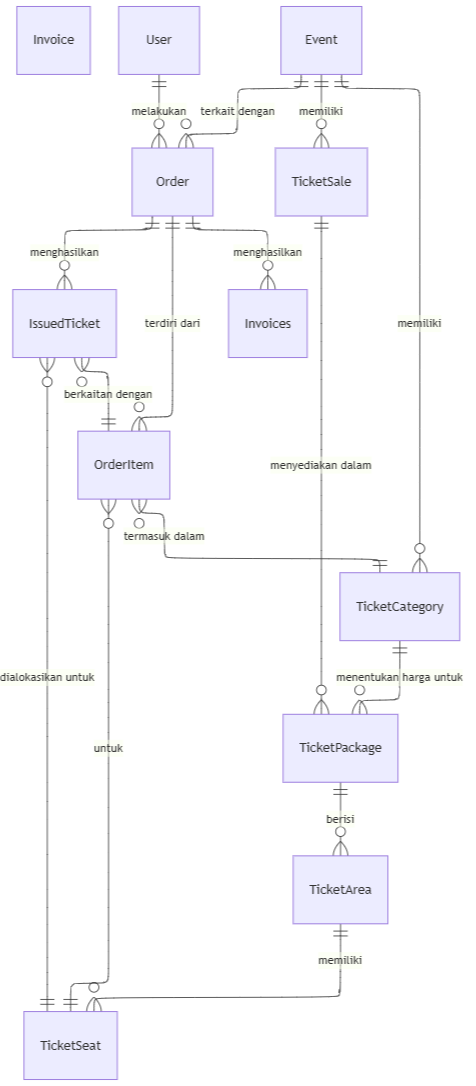
\includegraphics[width=0.7\textwidth]{resources/chapter-3/erd-mini.png}
    \caption{ERD Layanan Tiket}
    \label{fig:erd-ticket-service}
\end{figure}

\pagebreak

Sebuah acara bisa memiliki banyak kategori tiket, seperti tiket kategori reguler, gold, platinum. Setiap kategori tiket bisa meliputi banyak area, seperti tribun timur dan barat. Setiap area terdiri atas banyak Seat dengan status ketersediaan, yaitu tersedia, sedang dipesan, dan terjual.

Entitas TicketSale menunjukkan penjualan tiket yang dilaksanakan pada batas waktu tertentu. Hal ini untuk mengakomodasi penjualan tiket untuk suatu acara yang dilakukan beberapa kali, seperti penjualan tiket \textit{early bird} dan penjualan tiket untuk umum serta untuk mengakomodasi penjualan tiket untuk hari yang berbeda. Setiap TicketSale memiliki banyak TicketPackage yang menandakan kategori tiket yang dijual. Entitas ini terhubung dengan entitas TicketCategory dan memiliki atribut harga. Setiap Seat menunjukkan Seat (fisik) pada hari tertentu. Tiket Seat yang sama pada hari yang berbeda akan memiliki ID yang berbeda. IssuedTicket merupakan tiket yang telah berhasil terjual dan memiliki informasi pemilik tiket dan nomor seri tiket. Untuk menangani penjualan tiket tanpa nomor kursi, sistem membuat penomoran virtual yang akan dipasangkan secara otomatis saat pembelian.

Entitas yang berkaitan dengan pembelian tiket terdiri atas entitas User, Order, OrderItem, dan Invoice. Entitas Invoice ini menyimpan status tagihan yang memiliki berelasi dengan tagihan pada layanan pembayaran. Setiap pesanan terdiri atas banyak OrderItem. Entitas ini menyimpan informasi pemesan dan harga saat pembayaran.



\pagebreak

\subsection{Layanan Pembayaran}

Layanan ini merupakan perupaan sistem gerbang pembayaran eksternal. Layanan ini bukan gerbang pembayaran sesungguhnya, tetapi merupakan \textit{mock service} yang menyimulasikan alur gerbang pembayaran.

\subsubsection{Kebutuhan Fungsional}

Kebutuhan fungsional layanan pembayaran dibahas pada Tabel \ref{table:fungsional-pembayaran}.

\begingroup
\footnotesize
\begin{longtable}{|l|p{0.4\textwidth}|p{0.4\textwidth}|}
    \caption{Kebutuhan Fungsional Sistem Pembayaran}
    \label{table:fungsional-pembayaran}                                                                                                                                                                                                                                                                                                                                                                                                                   \\
    \hline
    \textbf{ID} & \textbf{Kebutuhan}                                                                                           & \textbf{Deskripsi}                                                                                                                                                                                                                                                                                                       \\
    \endfirsthead
    \multicolumn{3}{|l|}{\tablename\ \thetable\ -- \textit{Lanjutan dari halaman sebelumnya}}                                                                                                                                                                                                                                                                                                                                                             \\
    \hline
    \textbf{ID} & \textbf{Kebutuhan}                                                                                           & \textbf{Deskripsi}                                                                                                                                                                                                                                                                                                       \\
    \endhead
    \hline
    \multicolumn{3}{|r|}{\textit{Dilanjutkan ke halaman berikutnya}}                                                                                                                                                                                                                                                                                                                                                                                      \\
    \endfoot
    \hline
    \endlastfoot
    \hline
    PF-01       & Sistem dapat membuat tagihan pembayaran dan pranala pembayaran.                                              & Pembayaran dilakukan dengan mengirimkan permintaan kepada pranala yang diberikan dengan parameter sukses atau gagal. Selain itu, terdapat tenggat waktu pembayaran yang ditentukan berdasarkan parameter pada saat pembuatan tagihan. Pembayaran akan otomatis gagal apabila tidak dipenuhi hingga batas waktu tersebut. \\
    \hline
    PF-02       & Sistem memanggil \textit{webhook} yang telah ditentukan ketika terdapat pembayaran yang berhasil atau gagal. & Kebutuhan ini memastikan sistem dapat secara otomatis mengirimkan notifikasi ke sistem lain (seperti sistem tiket) setelah status pembayaran berubah.                                                                                                                                                                    \\
    \hline
    PF-03       & Sistem menyediakan \textit{endpoint} untuk menampilkan detail tagihan pembayaran.                            & Kebutuhan ini memungkinkan pengguna atau sistem lain untuk melihat rincian tagihan pembayaran, termasuk jumlah, tenggat waktu, dan statusnya.                                                                                                                                                                            \\
\end{longtable}
\endgroup

\subsubsection{Entitas Layanan}

Entitas yang berkaitan dengan layanan ini adalah entitas tagihan (Invoice). Properti entitas tagihan dibahas pada Tabel \ref{table:skema-invoice}.

\pagebreak

\begingroup
\footnotesize
\begin{longtable}{|l|p{0.4\textwidth}|p{0.4\textwidth}|}
    \caption{Skema Entitas Invoice}
    \label{table:skema-invoice}                                                                                           \\
    \hline
    \textbf{Atribut} & \textbf{Tipe Data}                     & \textbf{Deskripsi}                                        \\
    \hline
    \endfirsthead

    \multicolumn{3}{|l|}{\tablename\ \thetable\ -- \textit{Lanjutan dari halaman sebelumnya}}                             \\
    \hline
    \textbf{Atribut} & \textbf{Tipe Data}                     & \textbf{Deskripsi}                                        \\
    \hline
    \endhead

    \hline
    \multicolumn{3}{|r|}{\textit{Dilanjutkan ke halaman berikutnya}}                                                      \\
    \endfoot

    \hline
    \endlastfoot

    \hline
    id               & \texttt{string}                        & ID unik untuk setiap tagihan.                             \\
    \hline
    amount           & \texttt{number}                        & Jumlah total tagihan.                                     \\
    \hline
    description      & \texttt{string}                        & Deskripsi dari tagihan.                                   \\
    \hline
    externalId       & \texttt{string}                        & ID dari sistem eksternal yang terkait dengan tagihan ini. \\
    \hline
    createdAt        & \texttt{date}                          & Waktu saat tagihan dibuat.                                \\
    \hline
    expiredAt        & \texttt{date}                          & Waktu saat tagihan akan kedaluwarsa.                      \\
    \hline
    paidAt           & \texttt{date}                          & Waktu saat tagihan dibayar.                               \\
    \hline
    paidAmount       & \texttt{number}                        & Jumlah yang telah dibayarkan.                             \\
    \hline
    status           & "pending", "expired", "paid", "failed" & Status terkini dari tagihan.                              \\
    \hline
\end{longtable}
\endgroup
